\documentclass[tikz]{standalone}
\usepackage{tikz}
\usepackage{pgfplots}
\usepackage{amsmath,amssymb}
\usetikzlibrary{decorations}
\usetikzlibrary{decorations.pathreplacing, intersections, fillbetween}
\usetikzlibrary{calc,positioning}
\usetikzlibrary{plotmarks}
\usetikzlibrary{pgfplots.groupplots, pgfplots.colormaps}
\usepackage[T1]{fontenc}
\usepackage[scaled]{helvet}
\renewcommand\familydefault{\sfdefault}
\usepackage{sfmath}
\pgfplotsset{compat=newest, scale only axis, width = 11.5cm, height = 6.5cm}
\pgfplotsset{
    sciclean/.style={
        font=\footnotesize,
        axis background/.style={fill=white},
        axis on top=false,
        axis line style={-, black},
        tick align=inside,
        major tick length=0.15cm,
        grid=none,
        enlargelimits=false,
        title style={font=\small\bfseries, yshift=0.5em},
        label style={font=\footnotesize},
        tick label style={font=\scriptsize},
    }
}

\usepackage{xparse}
\NewDocumentCommand{\onslide}{s t+ d<>}{}
\NewDocumentCommand{\only}{d<>}{}
\NewDocumentCommand{\uncover}{d<>}{}
\NewDocumentCommand{\visible}{d<>}{}
\NewDocumentCommand{\invisible}{d<>}{}

\makeatletter
\tikzset{
Sloped/.code = {
\iftikz@fullytransformed%
    \tikzset{sloped}
\else
    \pgfgettransformentries{\mya}{\myb}{\myc}{\myd}{\mys}{\myt}%
    \tikzset{sloped, transform shape, rotate = {atan2(\myb,\mya)}}%
\fi
}
}
\makeatother

\definecolor{blue}{HTML}{0072BD}
\definecolor{orange}{HTML}{D95319}
\definecolor{yellow}{HTML}{EDB120}
\definecolor{purple}{HTML}{7E2F8E}
\definecolor{green}{HTML}{77AC30}
\definecolor{light-blue}{HTML}{4DBEEE}
\definecolor{red}{HTML}{A2142F}

\begin{document}
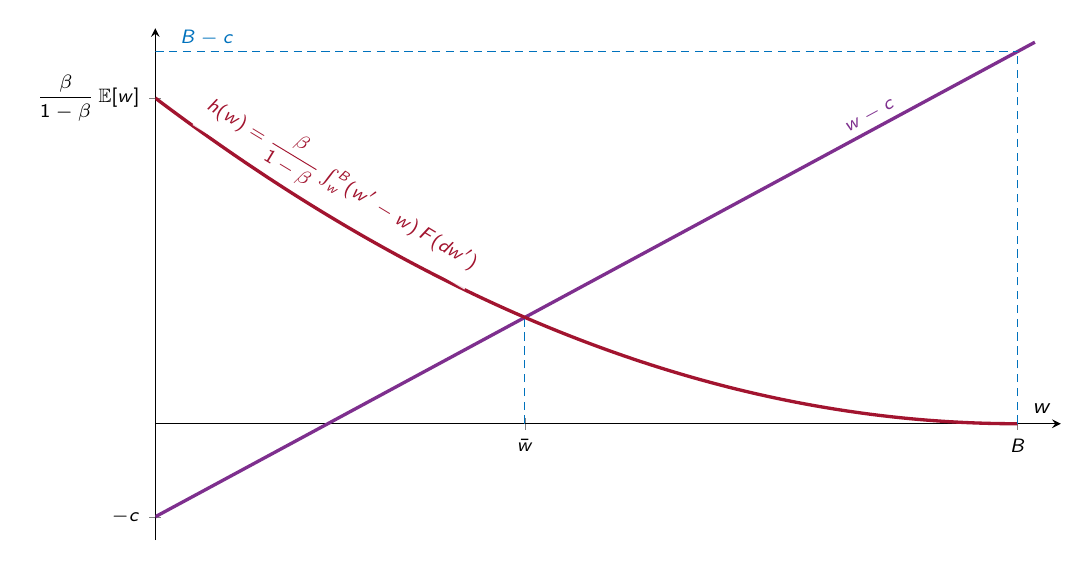
\begin{tikzpicture}

\begin{axis}[
    sciclean,
    axis lines=middle,
    axis x line*=middle,
    axis y line*=middle,
    xlabel={$w$},
    ylabel={},
    xmin=0, xmax=1.05,
    ymin=-0.25, ymax=0.85,
    xtick={0,0.428571,1},
    xticklabels={$0$, $\bar w$, $B$},
    ytick={-0.2,0,0.7},
    yticklabels={$-c$, $0$, $\dfrac{\beta}{1-\beta}\,\mathbb{E}[w]$},
]

% Parameters for drawing (normalized): c=0.2, B=1.
% LHS: w-c = x-0.2
% RHS: h(w) drawn as a decreasing convex curve: 0.7(1-x)^2
% Intersection is at \bar w = 3/7 \approx 0.4286.

% LHS line: w - c
\addplot[very thick, color=purple, domain=0:1.02, samples=2]
    {x - 0.2}
    node[pos=0.82, Sloped, above, font=\scriptsize,
         fill=white, fill opacity=0.85, text opacity=1, inner sep=1pt, yshift=1pt]
    {$w-c$};

% RHS curve: h(w)
\addplot[very thick, color=red, domain=0:1, samples=200]
    {0.7*(1-x)^2}
    node[pos=0.25, Sloped, above, font=\scriptsize,
         fill=white, fill opacity=0.85, text opacity=1, inner sep=1pt, yshift=2pt]
    {$h(w)=\dfrac{\beta}{1-\beta}\int_{w}^{B}(w'-w)\,F(dw')$};

% Vertical guide lines at \bar w and B
\addplot[densely dashed, color=blue] coordinates {(0.428571,0) (0.428571,0.228571)};
\addplot[densely dashed, color=blue] coordinates {(1,0) (1,0.8)};

% Horizontal guide at B-c
\addplot[densely dashed, color=blue] coordinates {(0,0.8) (1,0.8)}
    node[pos=0.06, above, font=\scriptsize,
         fill=white, fill opacity=0.85, text opacity=1, inner sep=1pt, yshift=1pt]
    {$B-c$};

\end{axis}
\end{tikzpicture}
\end{document}
